\documentclass[10pt]{article}
\usepackage[
  paperwidth=17.0cm,
  paperheight=5.2cm,
  margin=0.25cm
]{geometry}
\usepackage{tikz}
\usepackage{amsmath}
\usetikzlibrary{arrows.meta,calc,positioning}
\pagestyle{empty}
\setlength{\parindent}{0pt}

\definecolor{ink}{HTML}{25313C}
\definecolor{muted}{HTML}{65717C}
\definecolor{panel}{HTML}{F7F9FB}
\definecolor{linegray}{HTML}{7D8993}
\definecolor{cyanfill}{HTML}{D9F0F2}
\definecolor{orangefill}{HTML}{FBE2BF}
\definecolor{bluefill}{HTML}{DDE8F4}
\definecolor{greenfill}{HTML}{DCEFD8}
\definecolor{purplefill}{HTML}{E8E0F1}
\definecolor{accent}{HTML}{C94F45}
\definecolor{good}{HTML}{27824A}

\begin{document}
\noindent
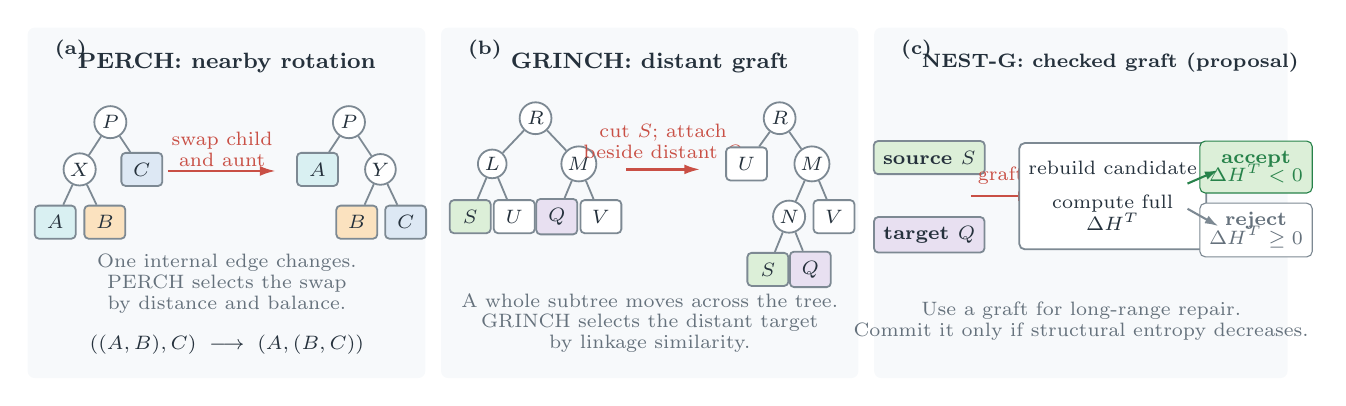
\begin{tikzpicture}[
  font=\sffamily,
  treeedge/.style={draw=linegray,line width=0.65pt},
  rootnode/.style={circle,draw=linegray,fill=white,inner sep=1.35pt,
                   line width=0.65pt,font=\scriptsize\bfseries,text=ink},
  internal/.style={circle,draw=linegray,fill=white,inner sep=1.1pt,
                   line width=0.65pt,font=\scriptsize,text=ink},
  leaf/.style={rounded corners=1.5pt,draw=linegray,minimum width=5.2mm,
               minimum height=4.2mm,line width=0.65pt,font=\scriptsize\bfseries,
               text=ink},
  flow/.style={-{Latex[length=2mm,width=1.25mm]},line width=0.85pt,draw=accent},
  smalllabel/.style={font=\fontsize{6.7}{7.5}\selectfont,text=muted,align=center},
  paneltitle/.style={font=\fontsize{8.2}{9}\selectfont\bfseries,text=ink},
  panellabel/.style={font=\fontsize{7.2}{8}\selectfont\bfseries,text=ink}
]

% Panel backgrounds.
\fill[panel,rounded corners=2.5pt] (0,0) rectangle (5.05,4.45);
\fill[panel,rounded corners=2.5pt] (5.25,0) rectangle (10.55,4.45);
\fill[panel,rounded corners=2.5pt] (10.75,0) rectangle (16.00,4.45);

% -------------------------------------------------------------------------
% (a) PERCH / rooted NNI.
\node[panellabel,anchor=west] at (0.22,4.17) {(a)};
\node[paneltitle,anchor=north] at (2.53,4.25) {PERCH: nearby rotation};

\node[rootnode] (ap1) at (1.05,3.25) {$P$};
\node[internal] (ax1) at (0.66,2.65) {$X$};
\node[leaf,fill=bluefill] (ac1) at (1.45,2.65) {$C$};
\node[leaf,fill=cyanfill] (aa1) at (0.35,1.98) {$A$};
\node[leaf,fill=orangefill] (ab1) at (0.98,1.98) {$B$};
\draw[treeedge] (ap1)--(ax1) (ap1)--(ac1) (ax1)--(aa1) (ax1)--(ab1);

\draw[flow] (1.78,2.63)--(3.15,2.63);
\node[smalllabel,text=accent] at (2.47,2.91) {swap child\\and aunt};

\node[rootnode] (ap2) at (4.08,3.25) {$P$};
\node[leaf,fill=cyanfill] (aa2) at (3.68,2.65) {$A$};
\node[internal] (ay2) at (4.48,2.65) {$Y$};
\node[leaf,fill=orangefill] (ab2) at (4.18,1.98) {$B$};
\node[leaf,fill=bluefill] (ac2) at (4.80,1.98) {$C$};
\draw[treeedge] (ap2)--(aa2) (ap2)--(ay2) (ay2)--(ab2) (ay2)--(ac2);

\node[smalllabel] at (2.53,1.20)
  {One internal edge changes.\\PERCH selects the swap\\by distance and balance.};
\node[smalllabel,text=ink] at (2.53,0.42)
  {$((A,B),C)\;\longrightarrow\;(A,(B,C))$};

% -------------------------------------------------------------------------
% (b) GRINCH graft.
\node[panellabel,anchor=west] at (5.47,4.17) {(b)};
\node[paneltitle,anchor=north] at (7.90,4.25) {GRINCH: distant graft};

% Before.
\node[rootnode] (br1) at (6.45,3.30) {$R$};
\node[internal] (bl1) at (5.90,2.72) {$L$};
\node[internal] (bm1) at (7.00,2.72) {$M$};
\node[leaf,fill=greenfill] (bs1) at (5.62,2.05) {$S$};
\node[leaf,fill=white] (bu1) at (6.18,2.05) {$U$};
\node[leaf,fill=purplefill] (bq1) at (6.72,2.05) {$Q$};
\node[leaf,fill=white] (bv1) at (7.28,2.05) {$V$};
\draw[treeedge] (br1)--(bl1) (br1)--(bm1)
  (bl1)--(bs1) (bl1)--(bu1) (bm1)--(bq1) (bm1)--(bv1);

\draw[flow] (7.60,2.65)--(8.54,2.65);
\node[smalllabel,text=accent] at (8.07,2.98) {cut $S$; attach\\beside distant $Q$};

% After.
\node[rootnode] (br2) at (9.55,3.30) {$R$};
\node[leaf,fill=white] (bu2) at (9.13,2.72) {$U$};
\node[internal] (bm2) at (9.96,2.72) {$M$};
\node[internal] (bn2) at (9.67,2.05) {$N$};
\node[leaf,fill=white] (bv2) at (10.24,2.05) {$V$};
\node[leaf,fill=greenfill] (bs2) at (9.40,1.38) {$S$};
\node[leaf,fill=purplefill] (bq2) at (9.94,1.38) {$Q$};
\draw[treeedge] (br2)--(bu2) (br2)--(bm2)
  (bm2)--(bn2) (bm2)--(bv2) (bn2)--(bs2) (bn2)--(bq2);

\node[smalllabel] at (7.90,0.70)
  {A whole subtree moves across the tree.\\GRINCH selects the distant target\\by linkage similarity.};

% -------------------------------------------------------------------------
% (c) Proposed entropy-certified use.
\node[panellabel,anchor=west] at (10.97,4.17) {(c)};
\node[paneltitle,font=\fontsize{7.2}{8}\selectfont\bfseries,anchor=north]
  at (13.75,4.25) {NEST-G: checked graft (proposal)};

\node[leaf,fill=greenfill,minimum width=8.5mm] (cs) at (11.45,2.80) {source $S$};
\node[leaf,fill=purplefill,minimum width=8.5mm] (cq) at (11.45,1.82) {target $Q$};
\draw[flow] (11.98,2.31)--(12.78,2.31);
\node[smalllabel,text=accent] at (12.36,2.57) {graft};
\node[draw=linegray,fill=white,rounded corners=2pt,minimum width=1.85cm,
      minimum height=1.35cm,align=center,font=\fontsize{7.2}{8}\selectfont,
      text=ink,line width=0.65pt] (score) at (13.78,2.31)
      {rebuild candidate\\[1.5mm]compute full\\$\Delta H^T$};
\node[draw=good,fill=greenfill,rounded corners=2pt,minimum width=8.5mm,
      minimum height=6.6mm,font=\fontsize{7}{8}\selectfont\bfseries,text=good,
      align=center]
      at (15.60,2.68) {accept\\[-0.5mm]$\Delta H^T<0$};
\node[draw=linegray,fill=white,rounded corners=2pt,minimum width=8.5mm,
      minimum height=6.6mm,font=\fontsize{7}{8}\selectfont\bfseries,text=muted,
      align=center]
      at (15.60,1.88) {reject\\[-0.5mm]$\Delta H^T\ge0$};
\draw[-{Latex[length=1.7mm,width=1.1mm]},line width=0.75pt,draw=good]
  (14.73,2.47)--(15.12,2.64);
\draw[-{Latex[length=1.7mm,width=1.1mm]},line width=0.75pt,draw=linegray]
  (14.73,2.15)--(15.12,1.93);

\node[smalllabel] at (13.38,0.72)
  {Use a graft for long-range repair.\\Commit it only if structural entropy decreases.};

\end{tikzpicture}
\end{document}
